\chapter{Ergebnisse}
\label{chap:ergebnisse} Dieses Kapitel präsentiert alle Ergebnisse, die in
dieser Arbeit erzielt wurde. Dabei spielen zunächst das Vorgehen eine Rolle, mit
der eine Bildbearbeitung durchgeführt werden kann. Gefolgt von einer Vorstellung
der entwickelten Software und deren Kernfunktionen. Anschließend wird auf die
Konzeptionen und Umsetzungen der verschiedenen Teile eingegangen. Diese bilden auch
gleichzeitig die Lösungen der einzelnen Teilaufgaben aus \ref{sec_zerlegung_in_teilprobleme}.
% ---------------------------------------------------------------------------------------

\section{Struktur und Aufbau der Software}
\label{sec:struktur_der_software} Bevor die Anwendung selbst mit ihrer Funktionalität
vorgestellt wird, ist es essenziell, zunächst die grundlegende Struktur offenzulegen,
auf der die Software basiert. Diese Struktur bildet das Fundament für die nachfolgenden
Implementierungsergebnisse, in denen sich viele ihrer Prinzipien und Konzepte
wiederfinden. Ein entscheidender Faktor für den erfolgreichen Entwicklungsprozess
war die enge Zusammenarbeit zwischen der Fachseite und den Softwareentwicklern.
Durch den kontinuierlichen Austausch zwischen Experten aus der medizinischen
Bildverarbeitung und der technischen Umsetzung konnte das Domänenwissen beider
Seiten optimal genutzt werden. Dies führte dazu, dass sowohl die spezifischen
Anforderungen der medizinischen Bildanalyse als auch die technischen
Möglichkeiten effizient in die Software einflossen.

Ein Besonders wichtiges Ergebnis dieser Zusammenarbeit ist die daraus
entstandene Struktur für die Bearbeitung von Mikro-\ac{CT}-Aufnahmen. Dieses
Vorgehen ist in der Abbildung \ref{fig:struktur_der_software} gezeigt und bildet
die Grundlage für alle weiteren Ergebnisse dieser Arbeit.

\begin{figure}[h]
	\centering
	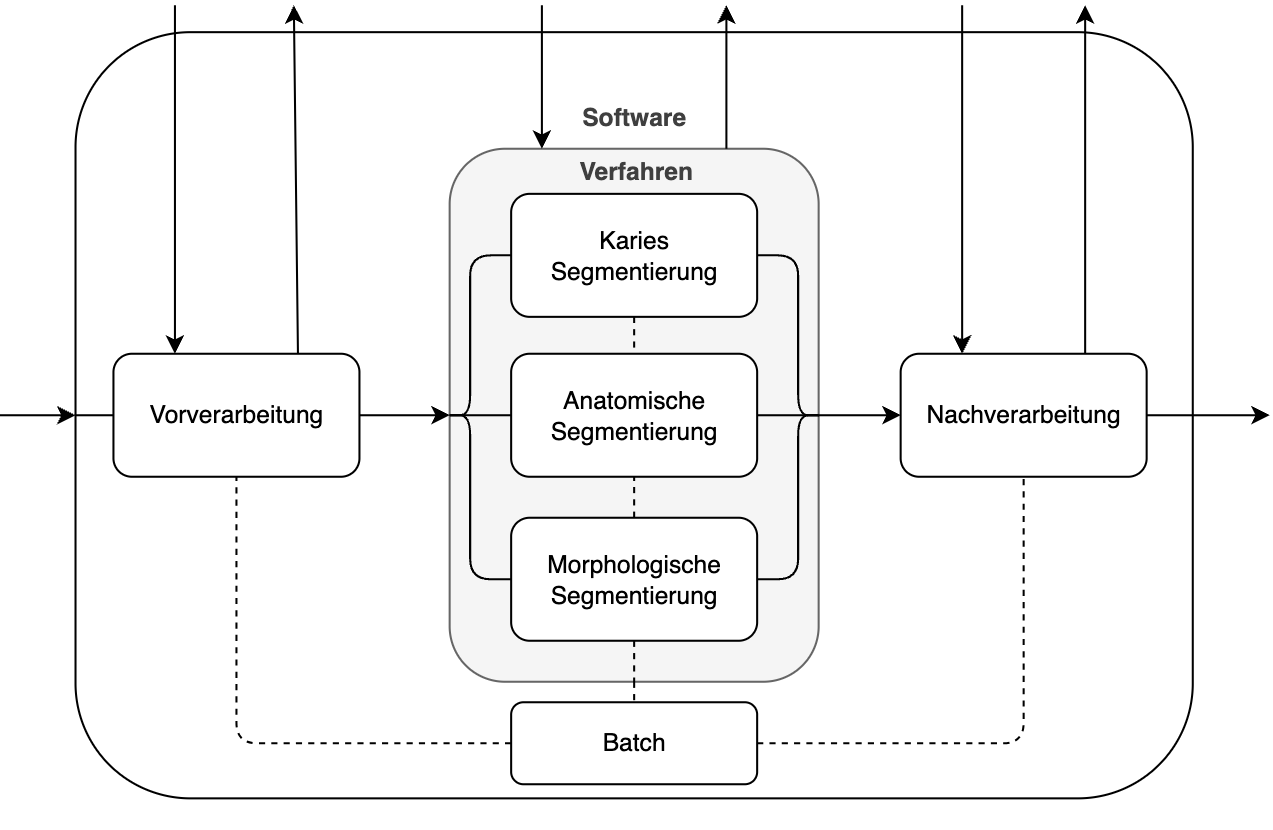
\includegraphics[width=0.8\textwidth]{img/struktur_der_software.png}
	\caption{Struktur der Software, die zusammen mit der Fachseite in der Klinik ausgearbeitet
	wurde (Pfeil: Mikro-CT-Datenstrom; Assoziation gestrichelt: abhängig)}
	\label{fig:struktur_der_software}
\end{figure}

Die Abbildung zeigt die Gesamtstruktur der entwickelten Software, die aus
mehreren Teilbereichen besteht. Diese lassen sich in einzelne Submodule unterteilen,
um eine klare funktionale Trennung zu gewährleisten. Die Software ist in drei zentrale
Verarbeitungsschritte gegliedert: die Vorverarbeitung, das eigentliche Verfahren
und die Nachverarbeitung des Mikro-\ac{CT}. Das dargestellte Verfahren umfasst verschiedene
Methoden zur Segmentierung, darunter die Karies-Segmentierung, die anatomische Segmentierung
und die morphologische Segmentierung. Diese Auswahl ist jedoch nicht
abschließend, sondern repräsentiert nur einige der möglichen Verarbeitungsmethoden.
Ein Mikro-\ac{CT} kann innerhalb einer Pipeline alle drei Verarbeitungsschritte in
festgelegter Reihenfolge durchlaufen (Vorverarbeitung, Bearbeitung,
Nachverarbeitung). Gleichzeitig hat die Forschung gezeigt, dass auch eine isolierte
Ausführung einzelner Schritte essenziell ist. Diese Flexibilität wird in der
Abbildung durch die verschiedenen Pfeilverbindungen verdeutlicht, die den Datenfluss
darstellen, von der Eingabe eines Mikro-\ac{CT} über die Verarbeitung bis hin zum
finalen Ergebnis. Neben der Einzelbildbearbeitung sollen alle diese gezeigten
Schritte auch in einem Batch-Prozess ausgeführt werden können. Dies sollen die gestrichelten
Assoziationen illustrieren. So kann Beispielsweise eine Vorverarbeitung isoliert
in einem Batch-Prozess durchgeführt werden. Unter der Vorverarbeitung eines Bildes
wird die Vorbereitung auf eine Verarbeitung verstanden. Dies könnte
beispielsweise eine Komprimierung der \ac{CT}-Aufnahme beinhalten. Das Kapitel
\ref{subsec:datensätze} Datensätze wies bereits auf eine enorme Größe der Mikro-\ac{CT}-Aufnahmen
hin und das diese dadurch schwer zu handhaben sind. Mittels Nachbearbeitung
könnten dann auf dem erzeugten Ergebnis Analysen durchgeführt werden. Durch Betrachtung
der Vor- und Nachverarbeitung anhand eines konkreten Beispiels, wird auch klar,
dass es durchaus sinnvoll ist, die geplanten Schritte auch einzeln auszuführen.

Auf dieser Basis wurde eine voll funktionsfähige Anwendung implementiert, die es
ermöglicht, Mikro-\ac{CT}-Bilder effizient zu analysieren und zu segmentieren. Im
Folgenden wird die entstandene Software im Detail vorgestellt, von der
Benutzeroberfläche über die zentralen Funktionen bis hin zu den technischen
Implementierungen.
% ---------------------------------------------------------------------------------------

\section{Tooth Analyser}
\label{sec:tooth_analyser} Im Rahmen dieser vorliegenden Arbeit ist eine Slicer
Erweiterung, entstanden, die den Namen Tooth Analyser trägt und für die
Forschung im Dentalbereich eingesetzt wird. In erster Linie können mit diesem Plug-in
Mikro-\ac{CT}-Aufnahmen anatomisch segmentiert werden. Das Modul schmiegt sich wie
alle anderen Module gut in die Kernanwendung ein und ist auch für die aktuelle stabile
Version von Slicer (v5.8.0) verfügbar. Neben der eigentlichen Implementierung
ist auch ein Logo für das Plug-in entstanden, das es nach außen repräsentiert.
Die Abbildung \ref{fig:logo_tooth_analyser} zeigt dies.

\begin{figure}[h]
	\centering
	
\includegraphics[width=0.8\textwidth]{img/SlicerToothAnalyser.png}
	\caption{Logo der 3D Slicer Erweiterung "Tooth Analyser", welche im Rahmen dieser
	Arbeit entwickelt wurde. Logodesign: Dr. Elias Walter}
	\label{fig:logo_tooth_analyser}
\end{figure}

Des Emblem des Tooth Analyser bildet einen Zahn ab, dessen Hauptsegmente (Schmelz,
Dentin, Pulpa) mit den unterschiedlichen Farben (grün, gelb, orange)
visualisiert werden. Dies verdeutlicht die Analogie zur anatomischen Segmentierung
und lässt gleich vermuten, dass sich dieses Modul mit einer Segmentierung
beschäftigt. Der Untertitel deutet konkret auf Mikro-\ac{CT}-Aufnahmen hin.

Wurde der Tooth Analyser installiert, so ist er über den Menüpunkt \textit{Module}
in Slicer auswählbar. Hier wird er in dem Unterpunkt \textit{Segmentierung}
eingruppiert, was ein weiteres Indiz auf die grobe Funktionalität liefert. Wird
also der Tooth Analyser gestartet so erhält man die Ansicht der Kernanwendung
mit der entsprechenden \ac{UI}. Die Abbildung \ref{fig:tooth_analyser_start_up}
soll genau diese Ansicht verdeutlichen.

\begin{figure}[h]
	\centering
	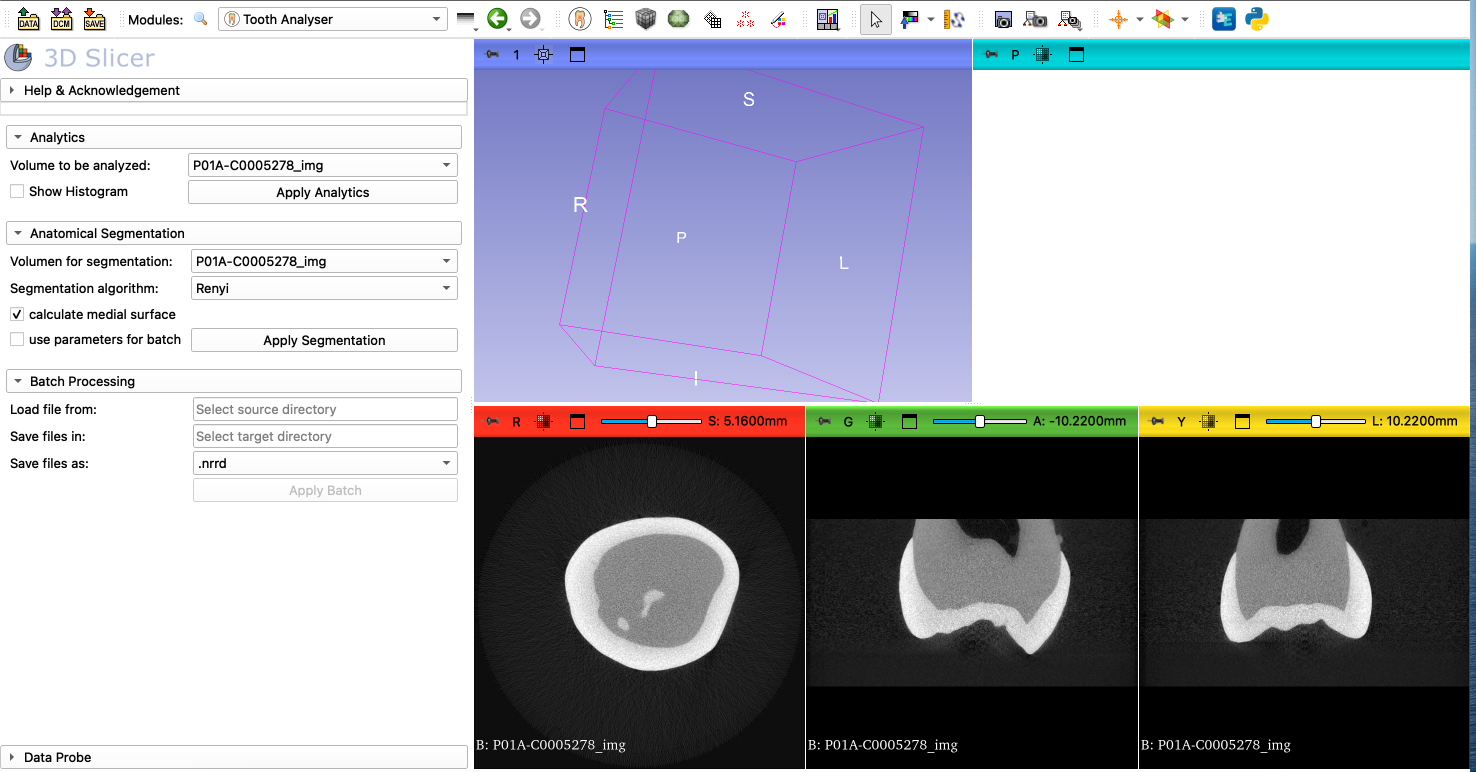
\includegraphics[scale=0.2, width=\textwidth]{img/toothAnalyserStarUp.png}
	\caption{Startansicht der Erweiterung Tooth Analyser bevor ein Verfahren
	gestartet wurde}
	\label{fig:tooth_analyser_start_up}
\end{figure}

Die Ansicht zeigt die Kernanwendung (rechts die verschiedenen Fenster) und die \ac{UI}
des jeweiligen Moduls. Die Kernanwendung kann auch als Szene beschrieben werden und
übernimmt alle generischen Handhabungen der Bilder. Neben den Szenen ist auch
immer eine Sidebar zu sehen, welche die \ac{UI} des jeweiligen Moduls abbildet. Im
Falle der Abbildung \ref{fig:tooth_analyser_start_up} ist es die \ac{UI} des
Tooth Analyser. Das manuelle Laden eines Bildes in die Szene ist Teil der Slicer
Kernanwendung und nicht Teil der Modullogik. Das bereits geladene Bild ist
demnach unabhängig vom der Tooth Analyser entstanden. Betrachtet man die Benutzerschnittstelle
genauer, so fällt sofort auf, dass diese in vier Bereiche unterteilt ist. Diese
Aufteilung in Bereiche ist ein Ergebnis der Recherche und dabei eine gute
Konvention in der Welt von 3D Slicer. Der Bereich \textit{Help and
Acknowledgement} stellt Hilfen und Informationen über das Modul bereit. Über diesen
Abschnitt ist auch die offizielle Dokumentation über dieses Modul erreichbar. Zu
beachten ist, dass dieser Bereich nicht eigens für den Tooth Analyser entwickelt
wurde. Es handelt sich hier um eine Funktionalität, die automatisch allen \ac{SEM}
zur Verfügung steht. Die übrigen Abschnitte sind Funktionen, die spezifisch für
den Tooth Analyser entwickelt wurden. Hier spiegelt sich auch der strukturelle Aufbau
wider, den der Tooth Analyser verfolgt und in Kapitel
\ref{sec:struktur_der_software} beschrieben wurde. Jede Funktionalität kann separat
ausgeführt werden. Bevor genauer auf die Funktionalitäten des Tooth Analyser
eingegangen wird, sei zunächst auf die Abbildung \ref{fig:tooth_analyser_full_view}
verwiesen, welche die Ergebnisansicht zeigt.

\begin{figure}[h]
	\centering
	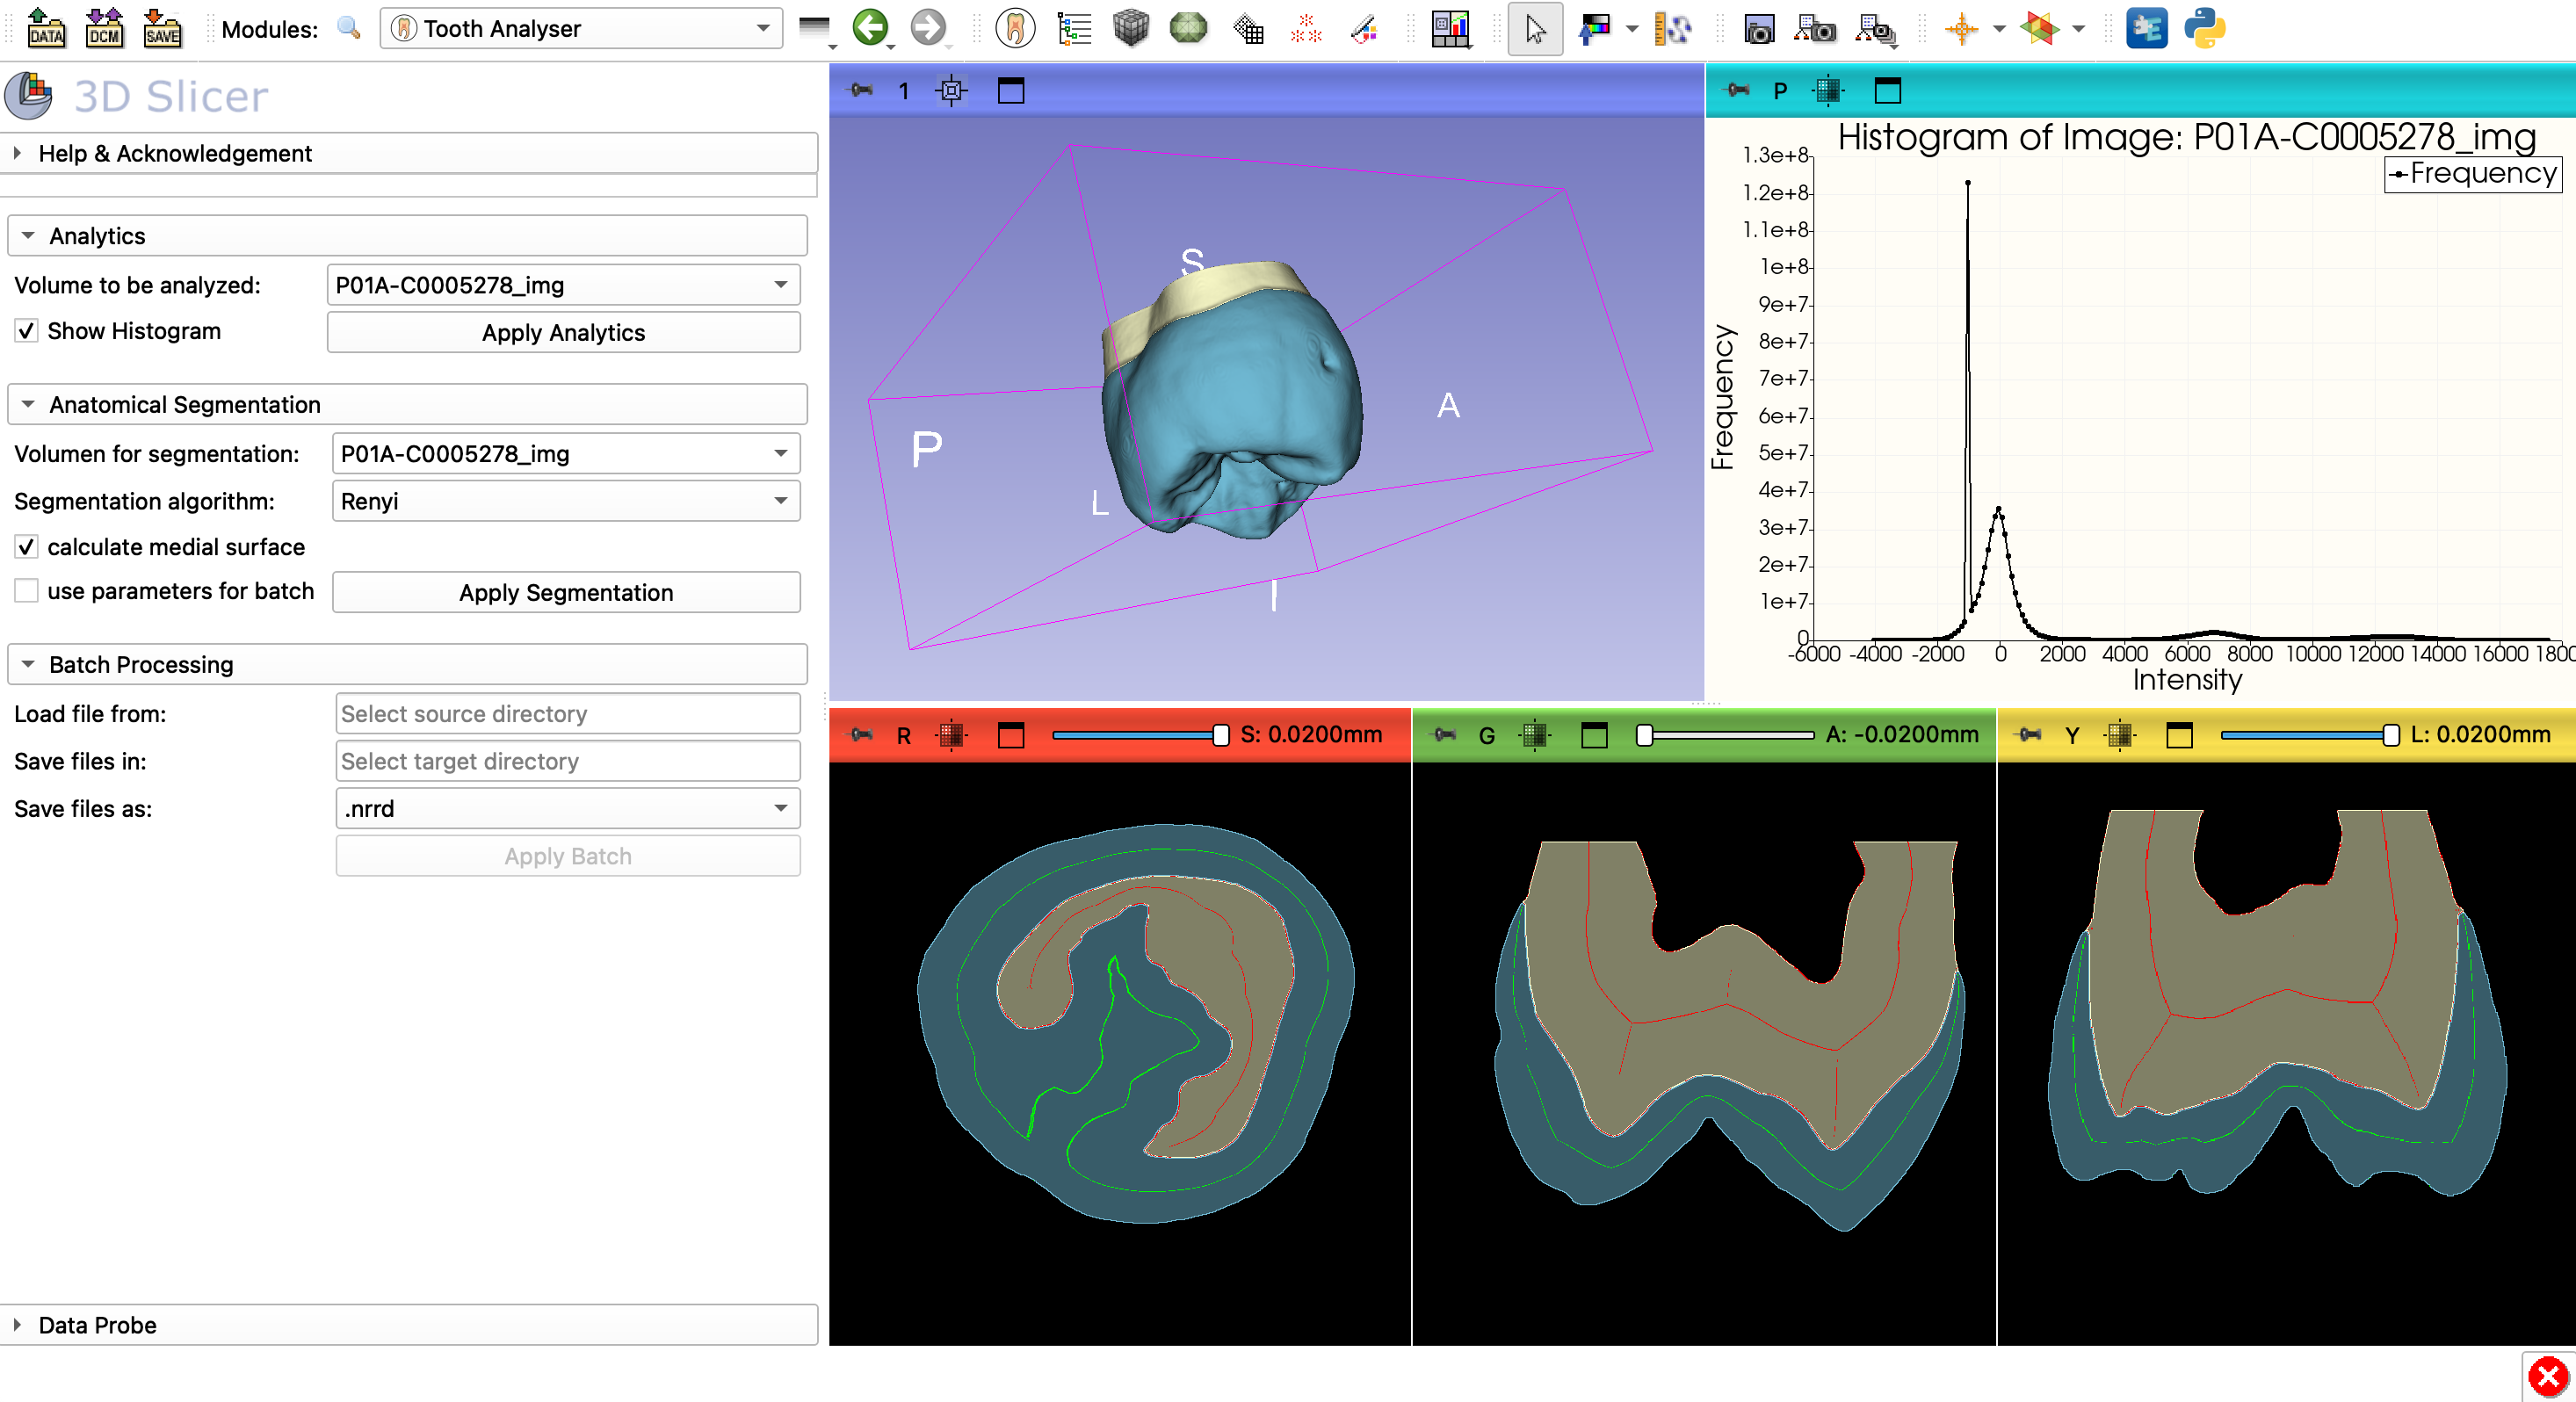
\includegraphics[scale=0.2, width=\textwidth]{img/toothAnalyserFullView.png}
	\caption{Ergebnisansicht der Erweiterung Tooth Analyser, nachdem die Analysen und
	die anatomische Segmentierung erstellt wurden}
	\label{fig:tooth_analyser_full_view}
\end{figure}

Der Analysebereich des Tooth Analyser ermöglicht es das Histogramm eines gegebenen
Bildes zu erstellen. Dies ist besonders interessant, wenn ein Algorithmus für die
anatomische Segmentierung ausgewählt werden muss. Diese Algorithmen sind
Schwellwertverfahren, die das Histogramm eines Bildes betrachten, um es zu
segmentieren. Das erstellte Histogramm ist rechts oben in der Abbildung \ref{fig:tooth_analyser_full_view}
zu erkennen. Es wird in einem \textit{Plot node} dargestellt und kann über diesen
auch verändert werden. Hierzu ist die Pinnnadel im Fenster des Plot-Knotens zu
wählen. Durch die Speicherfunktion der Kernanwendung kann der Plot auch problemlos
gespeichert werden. Bevor die Analysen erstellt werden können, müssen Parametereinstellungen
gewählt werden. Hierbei ist der wichtigste Parameter der, indem das konkrete Bild
ausgewählt wird. Bei diesem Parameter handelt es sich um ein Dropdown, indem nur
Bilder mit dem Typ \texttt{vtkMRMLScalarVolumeNode} ausgewählt werden können. Dies
trägt zur Stabilität und Ausfallsicherheit des Systems bei und sorgt dafür, dass
nicht jedes beliebige Bild geladen werden kann. Ist keine \ac{CT}-Aufnahme
ausgewählt, so bleibt der Button zum Starten der Analysen deaktiviert. Wird ein
Bild in die Szene geladen, während der Parameter für das zu analysierende Bild leer
ist, wählt der Tooth Analyser automatisch das Bild aus, dass als Erstes in die Szene
geladen wurde. So spart der Benutzer einige Klicks. Durch die Checkbox \textit{Show
Histogram} wird der Erweiterung signalisiert das beim Starten der Analysen ein
Histogramm des übergebenen Bildes erstellt werden soll.

Die Hauptfunktionalität des Tooth Analyser ist die anatomische Segmentierung
welche in Kapitel \ref{chap:theoretische_grundlagen} detailliert erläutert wurde.
Die konkreten Ergebnisse dieser Segmentierung sind in der Abbildung \ref{fig:tooth_analyser_full_view}
in den Fenstern (blau, rot, grün, gelb) zu sehen. Neben der eigentlichen Segmentierung
sind auch hier die medialen Flächen für die Segmente Dentin (rot) und Schmelz (grün)
gut sichtbar. Hinzu kommt ein \ac{3D} Modell, das auf Basis der erstellten
Segmentierung generiert wurde und nur der Visualisierung dient. Ein Abspeichern dieses
\ac{3D}-Modells als Netz ist nicht möglich. Um überhaupt eine anatomische Segmentierung
eines Zahnes erstellen zu können, sieht der Algorithmus zunächst drei Parameter
vor, die eingestellt werden müssen. Um die Komplexität gering zu halten, wurde bewusst
auf viele Parameter verzichtet. Ähnlich wie bei den Analysen ist auch hier die
Wahl des zu segmentierenden Volumens der entscheidende Parameter. Dessen Bedeutung
gleicht der Analysen, insbesondere in Bezug auf das Verhalten. Damit schnell ein
Ergebnis generiert werden kann, wurde für die übrigen zwei Parameter eine
Vorauswahl definiert, die zum vollen Ergebnisumfang des Tools führt. So ergibt
sich die Situation, dass nach dem Laden eines \ac{CT}s in die Szene nur auf den Button
für das Ausführen gedrückt werden muss, damit eine anatomische Segmentierung
erstellt wird. Dies nimmt dem Benutzer viel Arbeit ab und sorgt für eine gut \ac{UX}.
Sind jedoch Einstellungen in den Parametern gewünscht, so können diese natürlich
getätigt werden. Über den Parameter \textit{Segmentation algorithm} kann das
entsprechende Schwellwertverfahren gewählt werden, mit dem der Zahn segmentiert werden
soll. Dies mag nur geringfügig eine Änderung auf die Ergebnismenge ausmachen, kann
aber dennoch wichtig sein. Die Checkbox \textit{calculate medial surface} ermöglicht
eine optionale Erstellung der medialen Flächen. Wird diese Funktion ohnehin
nicht gebraucht, so kann diese hier ausgelassen werden und damit Laufzeit eingespart
werden.

Die letzte Funktionalität, die geboten wird, stellt kein neues Verfahren dar,
sondern nur eine andere Art der Ausführung. Die Rede ist hier von einem Batch Modus,
der nicht nur ein Bild segmentiert, sondern das Verfahren der anatomischen Segmentierung
auf eine ganze Reihe an Bildern anwendet. Um diesen Modus aktiv zu schalten, muss
neben den Parametern im Abschnitt \textit{batch} auch die Checkbox \textit{use
parameters for batch} aktiviert werden. Der Tooth Analyser überträgt dann die
aktuellen Parametereinstellungen der anatomischen Segmentierung an den Batch
Modus. Um dann den Batch Modus ausführen zu können, müssen noch zwei Pfade
angegeben werden, die jeweils zu einem Ordner führen. Diese beiden Pfade teilen
sich auf in \textit{source} und \textit{target} und geben an, wo die Daten liegen,
die segmentiert werden soll und wo die segmentierten Daten auf der Festplatte
gespeichert werden. Abschließend ist hier noch zu wählen in welchem Typ die erstellten
Daten abgespeichert werden sollen. Hierbei kann der Tooth Analyser zwischen den
Typen \ac{NRRD}, \ac{NIfTI} und \ac{MHD} unterscheiden. Bei diesem Feature ist zu
beachten, dass nach Erfolgreichem ausführen keine Daten in der Slicer Szene
geladen werden. Der Prozess läuft im Hintergrund und ist bis auf die Parametereinstellung
über die \ac{UI} komplett getrennt von Slicer. Nach Ende des Batch Modus wird in
dem angegebenen Zielordner ein Unterordner erstellt, der alle Dateien der
segmentierten Bilder enthält. Hierfür sieht der Tooth Analyser weitere Unterordner
für jedes segmentierte Bild vor. Ein automatisches Laden aller segmentierten
Bilder nach dem Batch Prozess ist nicht implementiert, sodass der erstellte Ordner
mit allen Segmentierungsdaten manuell über den Import geladen werden muss.

Wird nun eines der bereitgestellten Verfahren ausgeführt, so wechselt der Tooth
Analyser in einen sogenannten \textit{Processing Mode}. Dieser soll in erster
Linie dem Benutzer signalisieren, dass aktuell ein Prozess ausgeführt wird.
Hierzu sei auf die Abbildung \ref{fig:processing_mode} verwiesen.

\begin{figure}[h]
	\centering
	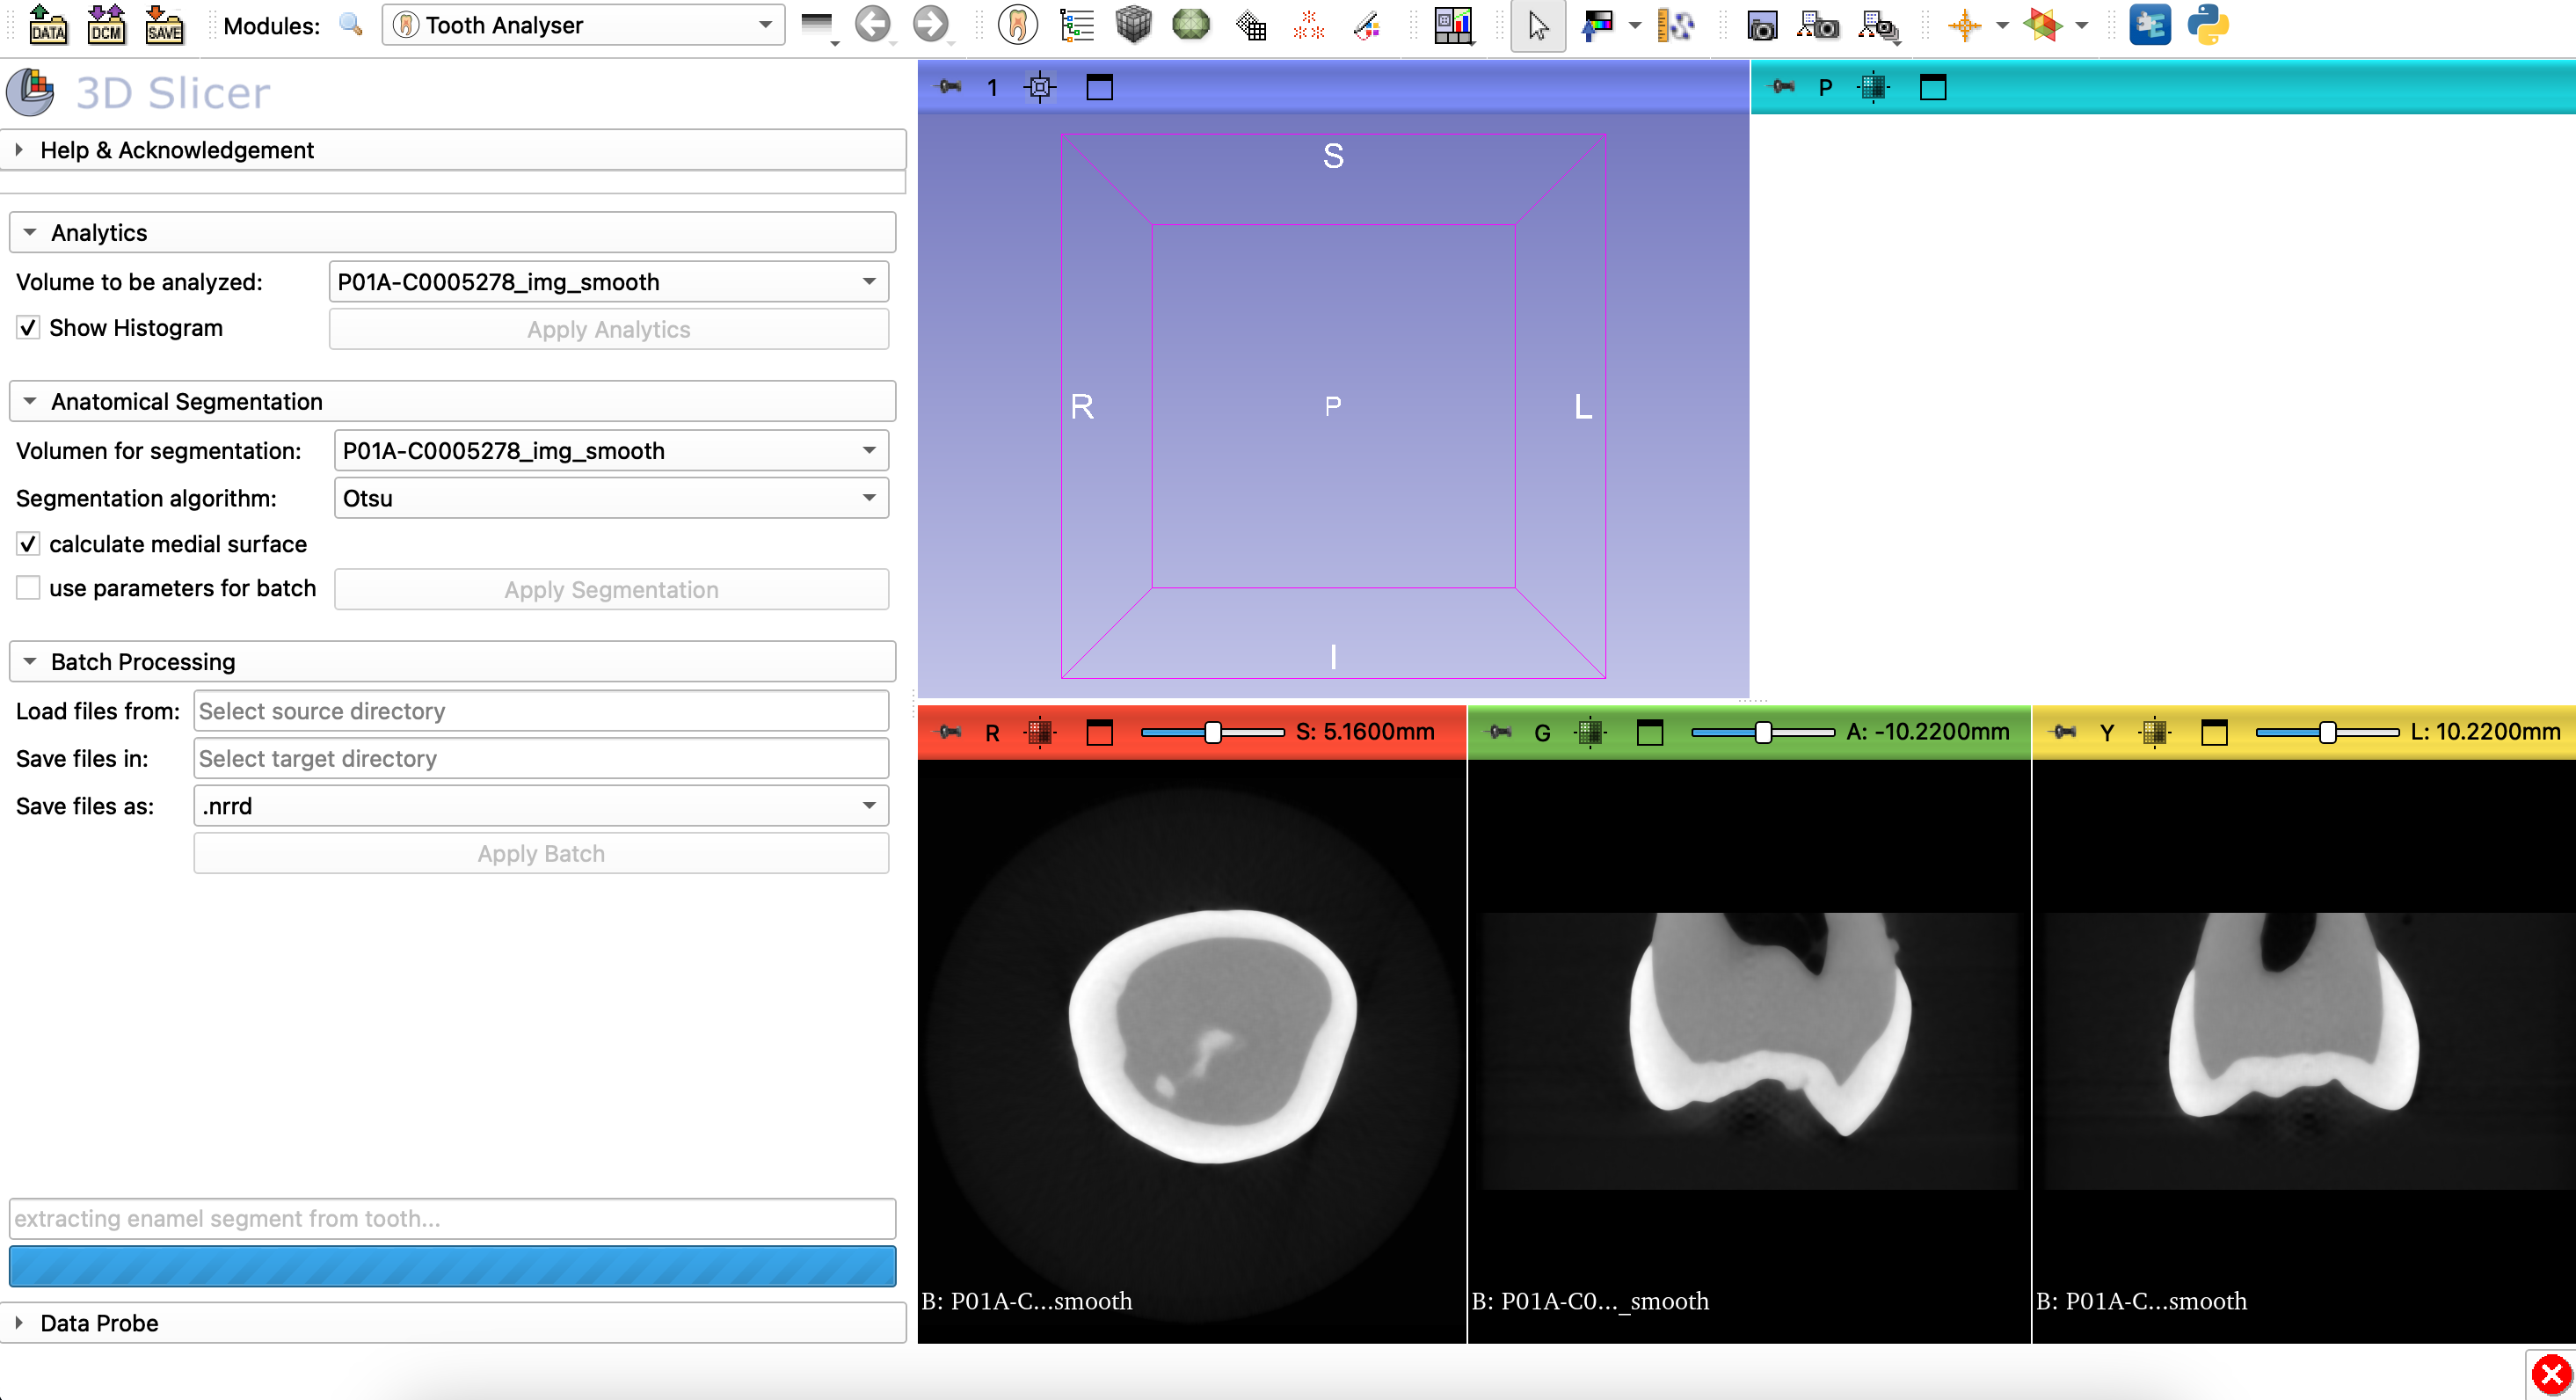
\includegraphics[scale=1, width=\textwidth]{img/processingMode.png}
	\caption{Ansicht des Moduls Tooth Analyser während der Ausführung eines
	Verfahrens}
	\label{fig:processing_mode}
\end{figure}

Mit dem Start eines Verfahrens wechselt der Tooth Analyser automatisch in einen Ausführungsmodus.
Dieser deaktiviert die Buttons zum Ausführen eines Algorithmus. Des Weiteren wird
am unteren Rand des Moduls eine Fortschrittsanzeige mit Statusleiste angezeigt,
um dem Benutzer mitzuteilen, in welchem Schritt er sich befindet. Der Cursor
ändert innerhalb der Anwendung dann den Modus auf "warten". Hierbei ist zu beachten,
dass Slicer selber während der Ausführung nicht bedient werden kann, da die Ressourcen
des Prozesses für den laufenden Algorithmus verwendet werden. Die Dokumentation
von Slicer empfiehlt hier auch kein parallelisieren der Anwendung, da dies zu \ac{GUI}
Fehlern führen würde. Der Benutzer muss also die Zeit abwarten. Treten während
der Bedienung der Software noch weitere Fehler auf, so verfügt der Tooth Analyser
auch über eine ausführliche Dokumentation. Diese ist im öffentlichen Repository
der Erweiterung einsehbar und in vier kleine Dokumentationen gegliedert \citep[vgl.][]{procida2017}.
Der Link zur Dokumentation ist dem Anhang zu entnehmen.

Da neben der reinen Erstellung noch weitere Anforderungen an die Erweiterung
gegeben waren, beschäftigt sich die nächsten Kapitel tiefer mit den softwaretechnischen
Aspekten des Tooth Analyser. Hierzu sollen auch die einzelnen Teilaufgaben, die zu
Beginn definiert wurden, wieder aufgegriffen werden.

\pagebreak
% ---------------------------------------------------------------------------------------

\section{Tooth Analyser Bibliothek}
Eine dieser Teilaufgaben beschäftigte sich mit der Integration der anatomischen Segmentierung
welches prototypisch als Python-Notebook bereitgestellt wurde. Dieses Notebook
funktioniert, war aber nicht gut strukturiert. So viel es schwer den Überblick
darin zu bewahren und das Verfahren gut nachzuvollziehen. Die gute Quelltextdokumentation
kompensiert dies etwas. Für das von Herrn Hofmann entwickelte Verfahren wurde
demnach ein eigenes Python-Modul erstellt. Somit konnte der Algorithmus von Aktivitäten
in Slicer gut getrennt werden. Das Verfahren selber wurde gut strukturiert in
Funktionen gekapselt, sodass schnell erkannt werden kann, in welchem Kontext
gerade gearbeitet wird. Die einfache Quelltextkommentierung wurde als Dokumentationsblock
an die jeweilige Funktion gehängt. Um die Einordnung des Moduls für die
anatomische Segmentierung besser einordnen zu können, sei die Projektstruktur hier
gezeigt.

\begin{lstlisting}[
    language={python},
    caption={Projektstruktur des Moduls Tooth Analyser mit Fokus auf die ToothAnalyserLib},
    label={lst:projektverzeichnis}]
|-- ToothAnalyser
|   |-- CMakeLists.txt
|   |-- Testing
|   |-- Resources
|   |-- ToothAnalyser.py
|   |-- ToothAnalyserLib
|   |   |-- NewFunction
|   |   |-- AnatomicalSegmentation
|   |   |   |-- __init__.py
|   |   |   |-- Segmentation.py
|   |   |   |-- isq_to_mhd.py
\end{lstlisting}

Zu sehen ist der Ordner \texttt{ToothAnalyser}, der alle Dateien beinhaltet, die
für das Modul relevant sind. Die Datei \texttt{TootAnalyser.py} ist das Hauptskript
und stellt die Anbindung an Slicer dar. Außerdem ist der Ordner \texttt{ToothAnalyserLib}
zu finden, der den ganzen externen Quellcode für das Modul beinhaltet, so auch die
anatomische Segmentierung. Kommen in Zukunft weitere Funktionen dazu, kann diese
Bibliothek problemlos um neue Funktionen erweitert werden. Dies symbolisiert der
Ordner \textsl{NewFunction}. Soll eine Funktion aus dieser Bibliothek verwendet
werden, so kann dies im Modul \texttt{ToothAnalyser.py} einfach über den
folgenden Befehl erfolgen.

\begin{lstlisting}[
    language={python},
    caption={Importieren von Funktionen aus der Bibliothek des Tooth Analyser},
    label={lst:tooth_analyser_lib}]
from ToothAnalyserLib.AnatomicalSegmentation.Segmentation import (loadImage, isSmoothed)
\end{lstlisting}

Betrachtet man das Python-Paket der anatomischen Segmentierung genauer, so fällt
auf, dass es sich in zwei Module teilt. Im Modul \texttt{Segmentation.py} befinden
sich alle Funktionen, die zum Ausführen der Pipeline für die anatomische
Segmentierung notwendig sind. Darüber hinaus finden auch einige Hilfsfunktionen Platz.
Das Modul \texttt{isq\_to\_mhd.py} liefert das Skript, mit dem Dateien im Format
\ac{ISQ} in eine \ac{MHD} Datei umgewandelt werden können. Die Verwendung der Methode
wurde bereits im Kapitel \ref{subsec:datensätze} Datensätze genauer beschrieben.
Für die Anwendung im Tooth Analyser wurde diese Methode leicht modifiziert.

\begin{lstlisting}[
    language={python},
    caption={Modifizierte Methode zum erstellen einer mhd-Datei aus einem ISQ-Format},
    label={lst:isq_mhd}]
def isq_to_mhd_as_string(isq_file_name) -> str:
    mhd_param, offset, grey_range = _read_isq_param(isq_file_name)
    mhd_param['ElementDataFile'] = isq_file_name

    # Use a StringIO buffer to construct the MHD content
    mhd_buffer = StringIO()
    for key, value in mhd_param.items():
        mhd_buffer.write(f"{key} = {value}\n")
    return mhd_buffer.getvalue()
\end{lstlisting}

Der Quellcode aus \ref{lst:isq_mhd} zeigt, dass statt einer Abspeicherung auf
der Festplatte ein Pufferspeicher genutzt wird (Zeile acht). Anstatt dann auf die
abgespeicherte Daten zu verweisen, wird einfach der Pufferspeicher ausgelesen (Zeile
neun).

Nachdem zu Beginn ein Gesamtüberblick über die Ergebnisse gewonnen wurde und
damit das Modul Tooth Analyser eingeführt wurde, folgen nun die Lösungen der restlichen
Teilaufgaben in Form von Implementierungsdetails.

\pagebreak
% ---------------------------------------------------------------------------------------

\section{Softwarekonzeptionen}
\label{sec:konzeptionen} Die ausgearbeiteten Konzeptionen bilden überwiegend die
Ergebnisse der in \ref{sec_zerlegung_in_teilprobleme} beschriebenen Teilaufgaben.
Konkret soll das bedeuten, dass hier konzeptionell gezeigt wird, wie die softwaretechnischen
Aspekte aus den Anforderungen umgesetzt wurden. Hierzu soll zunächst das Design-Klassendiagramm
betrachtet werden, das sich aus dem Domänenmodell in Abbildung \ref{fig:3d_slicer_domäne}
ableiten lässt. Zu beachten ist hier, dass es sich bei den Diagrammen in Abbildung
\ref{fig:klassendiagramm} und \ref{fig:klassendiagramm_new} um einen Ausschnitt handelt.
Das vollständige Design-Klassendiagramm ist dem Anhang zu entnehmen.

\begin{figure}[h]
	\centering
	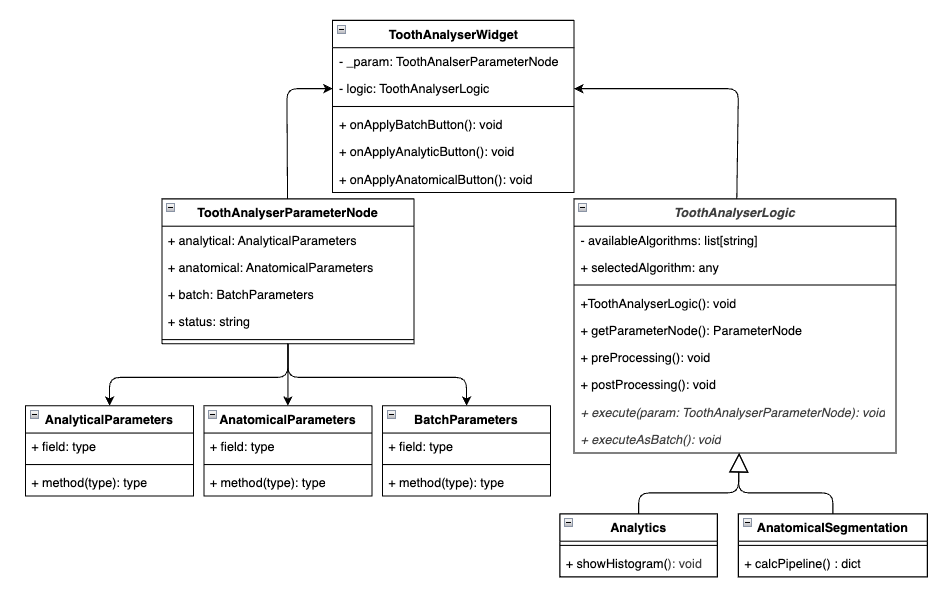
\includegraphics[width=0.9\textwidth]{
		img/tooth_analyser_class_diagram_light.png
	}
	\caption{Ausschnitt aus dem Klassendiagramm für den Tooth Analyser}
	\label{fig:klassendiagramm}
\end{figure}

Wie der weitere Verlauf des Kapitels zeigen wird, ist die Erweiterung unter
anderem über die Klassen \texttt{ToothAnalyserWidget} und \texttt{ToothAnalyserLogic}
in das Kernsystem eingebunden. Den Zentralen Punkt bildet dabei die Widget-Klasse.
Sie hält auf der einen Seite alle Parameter der verschiedenen Funktionen und auf
der anderen Seite die dazugehörigen Logiken. Des Weiteren bildet diese Klasse die
gesamt \ac{UI} des Tooth Analyser ab, was unter anderem das Laden der \ac{UI}
mit einschließt. Die \ac{UI} des Tooth Analyser wurde mit der Software QT-Designer
erstellt und dann mittels einer Methode in die Anwendung geladen. Wie auch schon
im Kapitel \ref{sec:tooth_analyser} beschrieben teilt sich die \ac{UI} auch hier
sichtbar in unterschiedliche Teile auf. Betrachtet man nun Abbildung \ref{fig:klassendiagramm}
so fällt auf, das für jeden Funktionsbereich eine eigene Parameterklasse
erstellt wurde, die dann wiederum in der Klasse ParameterNode zusammengefasst werden.
Dies stellt eine gute Erweiterbarkeit der \ac{UI} um zusätzliche Parameter sicher.
Es wurde an dieser Stelle bewusst keine Generalisierung verwendet, da Slicer genau
diesen konzeptionierten Mechanismus vorsieht. Auf der anderen Seite der Struktur
finden sich die Logikklassen. Die verschiedenen Logiken die aktuell und zukünftig
den Tooth Analyser ausstatten, verwenden alle dieselbe Schnittstelle, die über die
Klasse \texttt{ToothAnalyserLogic} bereitgestellt wird. Sollen also in Zukunft weitere
Funktionen hinzukommen, so kann hier einfach eine weitere Klasse an die
Schnittstelle angehängt werden. So entsteht etwas, das man in der Fachliteratur
als \textit{Strategy Pattern} bezeichnet \citep[vgl.][S.~99]{siebler2014}. Der Benutzer
der Software wählt also über die verschiedenen Buttons aus, welche Strategie er
gerade nutzen will. Der Tooth Analyser sorgt dann dafür, dass auch die richtige
Funktion geladen wird. Das Feature für den Batch Modus funktioniert nach einem anderen
Schema. Da dieser Modus auch für alle zukünftigen Funktionen gelten soll, wird dieser
nicht als eigene Strategie, sondern direkt in der Schnittstelle bereitgestellt. So
ist sichergestellt, dass eine Implementierung erfolgen muss, sie jedoch für alle
Strategien unterschiedlich sein kann. Um noch etwas genauer zu zeigen, welche Schritte
notwendig sind um den Tooth Analyser mit weiteren Funktionen auszustatten sei auf
Abbildung \ref{fig:klassendiagramm_new} verwiesen. Hier wird deutlich, welche Klassen
und Methoden erstellt werden müssen.

\begin{figure}[h]
	\centering
	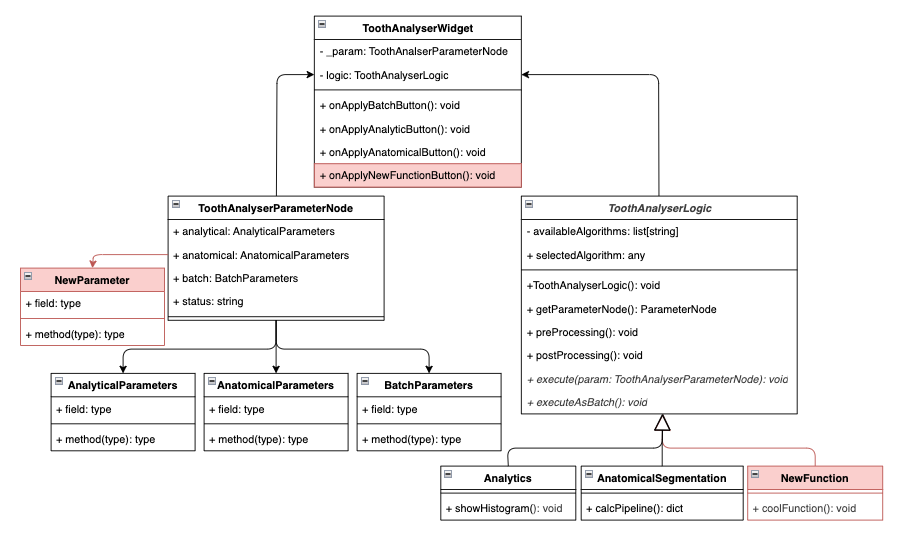
\includegraphics[width=0.9\textwidth]{
		img/tooth_analyser_class_diagram_new.png
	}
	\caption{Hinzufügen neuer Funktionen zum Tooth Analyser mittels des
	Klassendiagrammmausschnitts}
	\label{fig:klassendiagramm_new}
\end{figure}

Wie bereits zu erkennen ist, signalisieren die roten Elemente die Punkte, an
denen die Funktionalität erweitert werden kann. Um einen noch genaueren Einblick
in die Strukturen zu geben, geht das nachfolgende Kapitel noch einen Schritt
weiter und geht auf konkrete Implementierungsdetails ein.

\pagebreak
% ---------------------------------------------------------------------------------------

\section{Softwarearchitektur}
\label{sec:technische_umsetzung} Zu Beginn sei gesagt, dass dieses Kapitel nicht
alle Funktionen detailliert beschreibt, sondern sich auf die wichtigsten Funktionen
und Methode des Tooth Analyser beschränkt. Auf Basis des Klassendiagramms aus
Abbildung \ref{fig:klassendiagramm} lässt sich eine grobe Übersicht über die
wichtigsten Klassen gewinnen. Tabelle \ref{tab:methoden_klassen} fasst diese Übersicht
zusammen. Die Reihenfolge gibt eine grobe Orientierung bezüglich der Wichtigkeit.

\begin{table}[h]
	\centering
	\begin{tabular}{|c|c|c|}
		\hline
		\textbf{Klassen}             & \textbf{Beschreibung}                              \\
		\hline
		\texttt{ToothAnalyser}       & Klasse für den Abschnitt Hilfe                     \\
		\hline
		\texttt{ToothAnalyserWidget} & Die \ac{UI}-Klasse mit Anbindung an das Kernsystem \\
		\hline
		\texttt{ToothAnalyserLogic}  & Die Logik-Schnittstelle                            \\
		\hline
	\end{tabular}
	\caption{Wichtige Klassen und Methoden im Tooth Analyser, die von ScriptedLoadableModule
	erben}
	\label{tab:methoden_klassen}
\end{table}

Die drei Klassen aus der eben gezeigten Tabelle werden von der Slicer Dokumentation
grob vorgeschrieben, und bilden somit den Kern der Erweiterung. Alle drei erben von
der Klasse \texttt{ScriptedLoadableModule} und stellen so die Anbindung an das
Kernsystem sicher. Die Klasse \texttt{ToothAnalyser} bildet hierbei den
Abschnitt \textit{Help and Acknowledgemt}, den jedes Modul mitbringen muss. Dort
enthalten sind alle wichtigen Metainformationen über das konkrete Modul. Der
nachfolgende Ausschnitt eines Quelltextes zeigt grob den Aufbau dieser Klasse.

\begin{lstlisting}[
    language={python},
    caption={Grober Aufbau der Klasse ToothAnalyser nach der Slicer Dokumentation},
    label={lst:3d_slicer_test_class}]
class ToothAnalyser(ScriptedLoadableModule):
    def __init__(self, parent):
	    ScriptedLoadableModule.__init__(self, parent)
	    self.parent.title = _("ExtensionName")
	    self.parent.categories = ["categories"]
	    self.parent.dependencies = ["moduels"]
	    self.parent.contributors = ["author"]
	    self.parent.helpText = _("help")
	    self.parent.acknowledgementText = _("ackn.")
\end{lstlisting}

Direkt in Zeile eins ist zu sehen, dass die Klasse eine Generalisierung der
Klasse \texttt{ScriptedLoadableModule} ist. Über diese Elternklasse wird die
Integration in die Slicer Kernanwendung sichergestellt. Innerhalb des Konstruktors
der Klasse werden unterschiedliche Felder angelegt, welche die verschiedenen
Texte widerspiegeln sollen. Zu Beachten ist noch, dass die Felder die einen
einfachen String erwarten, in einer unscheinbaren Methode \texttt{\_()}
gekapselt sind. Diese Methode ist Teil des Slicer Python-Framework und sorgt dafür,
dass automatisch der Kontextname gewechselt wird. Über bekannte Html-Tags können
auch Bilder oder Hyperlinks eingebaut werden, welche auf Screenshots oder
Dokumentationen verweisen.

Die Klasse \texttt{ToothAnalyserWidget} bildet die gesamte Benutzerschnittstelle
der Erweiterung ab und kümmert sich gleichzeitig um das Zusammenspiel zwischen Logik
und Parameter. Hierfür hat die Widget-Klasse Zugriff auf alle Parameter und auf
die Logik-Schnittstelle. Das nachfolgende Listing zeigt einen groben Aufbau der Felder
innerhalb der Klasse \texttt{ToothAnalyserWidget}.

\begin{lstlisting}[
    language={python},
    caption={Verteilung der Felder in der Klasse Widget-Klasse},
    label={lst:create_ui}]
class ToothAnalyserWidget(ScriptedLoadableModuleWidget):
  def __init__(self, parent=None) -> None:
    ScriptedLoadableModuleWidget.__init__(self, parent)
    self.logic = None
    self._param = None
\end{lstlisting}

Wie auch schon die Klasse \texttt{ToothAnalyser} ist auch die Widget-Klasse eine
Kindklasse. Der Konstruktor dieser Klasse wird jedes Mal aufgerufen, wenn der
Benutzer zum ersten Mal nach dem Start von Slicer das Modul aufruft. Neben dem Konstruktoraufruf
der Elternklasse werden auch die Parameter und die Logik-Schnittstelle initialisiert.
So ergibt sich die Situation, dass die \ac{UI} die aktuellen
Parametereinstellungen abfragt und sie an die Logik weiterleitet.

Neben der Steuerungsaufgabe erstellt die Widget-Klasse auch die \ac{UI} aus der \ac{UI}-Datei
bereit. Da diese unter der Haube ein \ac{XML} Format aufweist, kann diese einfach
in das Modul hineingeladen werden. Der Quellcode aus \ref{lst:create_ui} zeigt
dies.

\begin{lstlisting}[
    language={python},
    caption={Laden der \ac{UI} in das Modul ToothAnalyser},
    label={lst:create_ui}]
def createUI(self) -> any:
  uiWidget = slicer.util.loadUI(self.resourcePath("UI/W.ui"))
  self.layout.addWidget(uiWidget)
  self.ui = slicer.util.childWidgetVariables(uiWidget)
  return uiWidget
\end{lstlisting}

Mittels der Bibliothek \texttt{slicer} lässt sich hier die Datei für die \ac{UI}
laden. Diese Datei liegt im Ordner \textit{Resources} sodass der Pfad zu diesem Ordner
mit der Methode \texttt{self.resourcePath()} ausgelesen werden kann. Als Argument
kann dann der Name der Datei angegeben werden. In diesem Fall existiert noch ein
Unterordner mit der entsprechenden Datei (\texttt{"UI/W.ui"}).

Ein weiterer nennenswerter Punkt in der Klasse \texttt{ToothAnalyserWidget} sind
die eventbasierten Methoden. Diese sorgen dafür, dass auf bestimmte Aktionen in
der Anwendung reagiert werden kann. Der Tooth Analyser hat in der Widget-Klasse mehrere
solcher Event-Methoden, die hier genannt werden.

\begin{description}
	\item[enter(),] wird immer ausgeführt, wenn der Benutzer das Modul öffnet

	\item[exit(),] wird immer ausgeführt, wenn der Benutzer ein anderes Modul
		öffnet

	\item[onSceneStartCloes(),] wird immer ausgeführt, kurz bevor das Modul
		geschlossen wird

	\item[onSceneEndClose(),] wird ausgeführt, nachdem das Modul geschlossen wurde

	\item[observeParameter(),] wird ausgeführt, wenn der Benutzer Änderungen an
		der \ac{UI} macht
\end{description}

Die Methode \texttt{observerParameter()} ist hierbei sehr interessant und
verdient besondere Betrachtung. Die Methode ist eine Beobachtungsmethode, die an
ein Event gekoppelt ist, dass sich \textit{ModifiedEvent} nennt. Dieses Event wird
immer ausgelöst, wenn der Benutzer Änderungen in der Slicer \ac{UI} macht. Dies
umschließt nicht nur das Modul. Wird also solch ein Event gefeuert, so wird die
Methode \texttt{observeParameter()} aufgerufen. Das Listing
\ref{lst:observe_parameter} zeigt diese Methode:

\begin{lstlisting}[
    language={python},
    caption={Methode zum Beobachten von Änderungen in der Benutzerschnittstelle},
    label={lst:observe_parameter}]
def observerParameters(self, caller=None, event=None)->None:
  self.handleApplyBatchButton()
  self.handleApplyAnalyticsButton()
  self.handleApplyAnatomicalButton()
\end{lstlisting}

Die Methode verfügt über die Parameter \texttt{caller} und \texttt{event}.
Mittels diesen Parametern kann der Auslöser des Events und die Art des Events
bestimmt werden. So könnte man verschiedenen Aktionen auf verschiedene Events ausführen.
Innerhalb des Tooth Analyser wird diese Methode genutzt, um die Klick-Logik der Buttons
abzubilden. Die Methoden \texttt{handleApply<...>Button()} steuern jeweils die Sichtbarkeiten
der einzelnen Buttons. Immer wenn der Benutzer dann Änderungen an der \ac{UI} durchführt,
wird die Logik innerhalb dieser Methode aus Listing \ref{lst:observe_parameter}
aktualisiert.

Die letzte der wichtigen Klassen bildet die Logik-Schnittstelle, wie sie in Tabelle
\ref{tab:methoden_klassen}, Zeile drei genannt wurde. Diese Schnittstelle ist der
zentrale Punkt aller aktuellen und zukünftigen Logikklassen. Jede Klasse, die einen
speziellen Algorithmus implementiert, muss dieses Interface implementieren. So wird
sichergestellt, dass alle Algorithmen nach dem gleichen Aufbau eingebaut werden.
Dies sorgt für ein einheitliches Vorgehen. Das Listing \ref{lst:logik_interface}
zeigt diese eben beschriebenen Schnittstelle und soll diese so genauere
beleuchten.

\pagebreak

\begin{lstlisting}[
    language={python},
    caption={Die Logik-Schnittstelle des Tooth Analyser},
    label={lst:logik_interface}]
class ToothAnalyserLogic(ScriptedLoadableModuleLogic):
    def __init__(self) -> None:
        ScriptedLoadableModuleLogic.__init__(self)

    def getParameterNode(self) -> ToothAnalyserParameterNode:
        return ToothAnalyserParameterNode(super().getParameterNode())

    def preProcessing(self) -> None:
        """Implement pre processing here"""
        pass

    def postProcessing(self) -> None:
        """Implement post processing here"""
        pass

    def execute(self, param: ToothAnalyserParameterNode)->None:
        """Abstract method"""
        raise NotImplementedError("Please implement this")

    def executeAsBatch(self, param: ToothAnalyserParameterNode)->None:
        """Abstract method"""
        raise NotImplementedError("Please implement this")
\end{lstlisting}

Auch die dritte der wichtigen Klassen erbt von einer übergeordneten Klasse und
verfügt so über deren Funktionen. Die Schnittstelle verfügt über drei Methoden,
die eine Standardimplementierung haben und direkt im Interface implementiert
werden. Die Methode \texttt{getParameterNode()} sorgt dafür, dass alle Parameter
des Moduls zur Verfügung stehen und verwendet werden können. \texttt{preProcessing()}
und \texttt{postProcessing()} sind für eine Vor- und Nachverarbeitung des entsprechenden
Bildes verantwortlich. Die Vorverarbeitung könnte beispielsweise eine
Komprimierung des Bildes beinhalten, wohingegen die Nachbereitung Analysen auf dem
Ergebnis anstoßen könnte. Im Rahmen dieser vorliegenden Arbeit wurden für die
Methoden \texttt{preProcessing()} und \texttt{postProcessing()} keine
Methodenrümpfe gebaut. Eine mögliche zukünftige Implementierung ist im Kapitel \ref{chap:schlussfolgerung}
zu finden. Die beiden noch übrigen Methoden \texttt{execute()} und \texttt{executeAsBatch()}
sind abstrakte Methoden, die eine Implementierung in den jeweiligen Unterklassen
erfordern. Dabei bilden beide Methoden zentrale Punkte. Innerhalb dieser Methoden
soll der entsprechende Algorithmus der Klasse ausgeführt und gestartet werden.
Einmal mit nur einem Bild und anschließender Visualisierung in der Slicer Szene
und einmal als Batch ohne Visualisierung.

Neben den drei Hauptklassen, die auch die Integration in das Kernsystem von 3D Slicer
sicherstellen, verfügt der Tooth Analyser auch über einen Mechanismus, der die Kommunikation
zwischen der Benutzerschnittstelle und dem Quellcode der Erweiterung realisiert.
Für das Erstellen einer \ac{UI}, die für eine Slicer Erweiterung notwendig ist, nutzt
3D Slicer den Qt-Designer \citep[vgl.][]{qt2024}. Die Integration des Qt-Designers
als Applikation in eine andere Applikation funktioniert aufgrund der Plattformintegrität,
die der Designer mitbringt \citep[vgl.][]{qt2024}. Diese bietet so die
Möglichkeit die benötigten Widgets über eine interaktive Benutzerschnittstelle
zu bauen. Für diese \ac{UI}-Vorrichtung gibt es einen Gegenspieler im Quelltext
des Programmes, welcher als \textit{ParameterNode} bekannt ist. Der \textit{ParameterNode}
ist laut \citet{slicer2024} eine leichte Variante eines \ac{MRML}-Knoten um
Parametereinstellungen zu speichern. Durch das Zusammenspiel zwischen \ac{UI}
und \textit{ParameterNode} wird die \ac{UI} automatisch aktualisiert, wenn sich das
Programm ändert \citep[vgl.][]{slicer2024}.

Das Erstellen der Verknüpfung zwischen \ac{UI}-Widget und \textit{ParameterNode}
erfolgt über die dynamische Eigenschaft \texttt{SlicerParameterName}, die direkt
in der Komponentenansicht im Qt-Designer einstellbar ist. Die Abbildung \ref{fig:qt_designer}
soll diesen Vorgang verdeutlichen. Dabei ist es wichtig, dass genau diese Eigenschaft
auch verwendet wird. Diese Verknüpfung lässt sich laut \citet{slicer2024} auch via
Programmcode setzten.

\begin{minipage}{0.55\textwidth}
	\centering
	\begin{lstlisting}[
		language=Python,
		label={lst:qt_parameter_node},
		caption={Ausschnitt des Parameter Knoten im Quellcode des Tooth Analysers, der mit der UI über den Parameter \texttt{SlicerParameterName} gekoppelt ist}]
@parameterNodeWrapper
class ToothAnalyserParameterNode:
    batch: Batch
    status: str = ""
    \end{lstlisting}
\end{minipage}
\hfill
\begin{minipage}{0.35\textwidth}
	\centering
	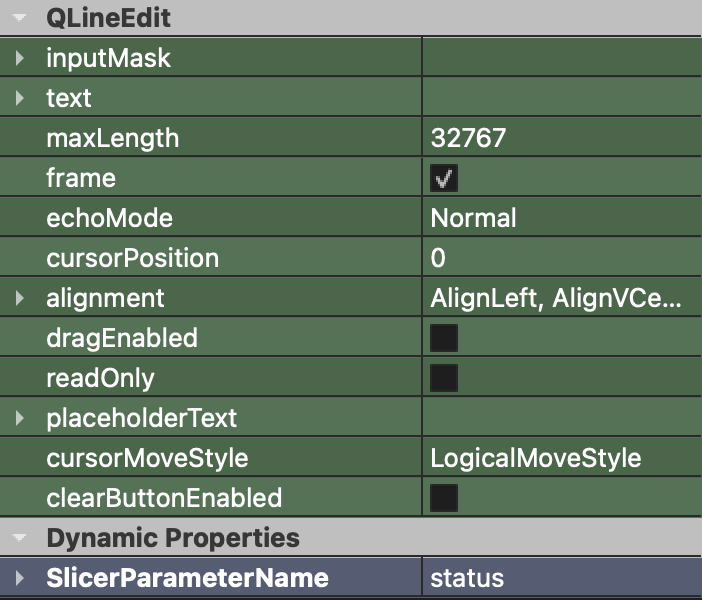
\includegraphics[width=\textwidth]{img/qt_designer.png}
	\captionof{figure}{Komponentenansicht der Komponente status im QT-Designer} \label{fig:qt_designer}
\end{minipage}

Betrachtet man erst das Feld \texttt{status} im Quellcode \ref{lst:qt_parameter_node}
und dann den Parameter \texttt{SlicerParameterName} in der Abbildung
\ref{fig:qt_designer}, so fällt auf, dass diese einheitliche Benennung die \ac{UI}
mit dem Quellcode verbindet. Dabei ist es wichtig, das genau dieser Parameter Name
für die dynamische Eigenschaft verwendet wird.

Nachdem die Implementierung der wichtigsten Komponenten isoliert besprochen wurden,
soll der Abschluss des Kapitels noch genauer beleuchten, wie die unterschiedlichen
Klassen und Komponenten untereinander interagieren.

Um die Architektur des Tooth Analyser noch genauer nachvollziehen zu können,
soll abschließend in diesem Kapitel das Zusammenspiel genauer betrachtet werden.
Hierbei geht es um die Abfolge von Methoden, die zum Starten eines Verfahrens
notwendig sind. Dafür sei auf die drei nachfolgenden Quellcodeblöcke verwiesen,
die jeweils einen Teilbereich an Funktionalität bereitstellen.

Zu Beginn werden in \ref{lst:parameter_node} die Parameter angelegt. Diese können
sich noch in weitere Klassen aufteilen, sodass die Parameter unterschiedlicher
Funktionen in unterschiedlichen Klassen zu finden sind. Siehe auch \ref{fig:klassendiagramm}
Klassendiagramm.

\begin{lstlisting}[
    language={python},
    caption={Die Parameter des Tooth Analyser, die als Attribut in der Widget-Klasse liegen},
    label={lst:parameter_node}]
@parameterNodeWrapper
class ToothAnalyserParameterNode:
    analytical: AnalyticalParameters
    anatomical: AnatomicalParameters
    batch: Batch
    status: str = ""
\end{lstlisting}

Die Klasse \texttt{ToothAnalyserParameterNode} speichert die Benutzereinstellungen
und ist mit der UI-Datei aus dem QT-Designer gekoppelt. Um diese Kopplung
herzustellen wird die Klasse mit dem \textit{Decorater} \texttt{@parameterNodeWrapper}
versehen. Die Klasse \texttt{ToothAnalyserWidget} hat vollen Zugriff auf die
Parameter Klasse und kann sie verwenden. Diese Verwendung ist in \ref{lst:on_apply}
zu sehen.

\begin{lstlisting}[
    language={python},
    caption={Starten des Algorithmus durch den Aufruf der \texttt{execut()} Methode in der Widget-Klasse. Die Parameter werden mit übergeben},
    label={lst:on_apply}]
def onApplyAnatomicalButton(self) -> None:
    self.activateComputingMode(True)
    with slicer.util.tryWithErrorDisplay(_("Failed")):
	  try:
	    AnatomicalSegmentationLogic.execute(self._param)
	  except:
	    slicer.util.errorDisplay(_("Error"))
    self.activateComputingMode(False)
\end{lstlisting}

Mit dem Zugriff auf die Parameter kann die Widget-Klasse den entsprechenden
Algorithmus starten und die Parametereinstellungen dafür übergeben. Dies wird in
der Methode \texttt{onApply()} realisiert, welche in der Klasse \texttt{ToothAnalyserWidget}
liegt. Die Methode sorgt außerdem dafür, dass der Algorithmus in einer sicheren
Umgebung gestartet wird. Sollte es bei der Ausführung zu unerwarteten Fehlern kommen,
so bricht der Tooth Analyser den Vorgang mit einer Fehlermeldung ab. Um die Ausführung
in der entsprechenden Logikklasse genauer zu betrachten, sei hier auf den
nachfolgenden Quellcode verwiesen.

\begin{lstlisting}[
    language={python},
    caption={Ein Ausschnitt der Methode \texttt{execute()}, welche die Pipeline für das Verfahren startet und in der Widget-Klasse durch den Apply-Button aufgerufen wird},
    label={lst:execute}]
@classmethod
def execute(cls, param: ToothAnalyserParameterNode) -> None:
    toothDict = cls.calcPipeline(
	    sourcePath=sourcePath,
	    calcMidSurface=param.anatomical.calcMidSurface,
	    param=param,)
\end{lstlisting}

Die Methode \texttt{execute()} aus \ref{lst:execute}, welche die Schnittstelle vorschreibt,
bekommt die Parametereinstellungen des Benutzers über das Argument. Somit ist während
der Ausführung ein voller Zugriff auf die Parameter gewährleistet. Ist die
Methode \texttt{execute()} vollständig durchgelaufen, so kommt das Verfahren zum
Ende.

Fasst man dieses Vorgehen kurz zusammen, lässt sich sagen, dass die Parameter, die
im Parameter Knoten gespeichert werden wie bereits beschrieben als Attribut in der
Klasse \texttt{ToothAnalyserWidget} liegen. Wenn ein Button zum Ausführen der entsprechenden
Logik gedrückt wird, wird die Methode \texttt{execute()} ausgeführt und alle Parameter
als Argument mit übergeben.

Nach der konkreten Umsetzung der Erweiterung und der Implementierungsdetails,
kann Schritt für Schritt mit der Evaluation der Ergebnisse begonnen werden. Ein wichtiger
Teil sind die Testergebnisse.
% ---------------------------------------------------------------------------------------